\section{Estimation} \label{sec:estimation}

\begin{figure*}
\subfloat[\label{fig:gp_r2_latency}]{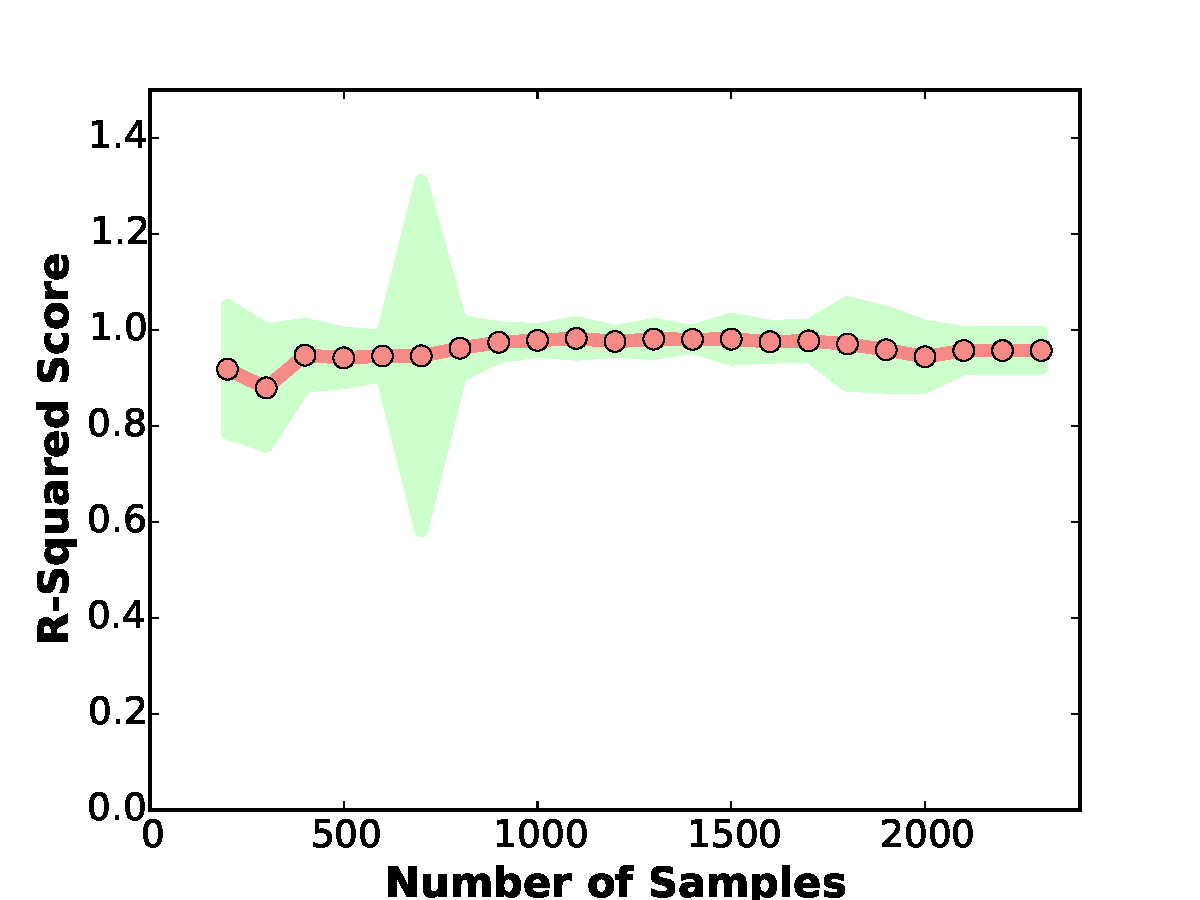
\includegraphics[width=0.5\textwidth]{figure/gp_per_benchmark_r2_scores_latency_mutate.pdf}} %
\subfloat[\label{fig:gp_r2_throughput}]{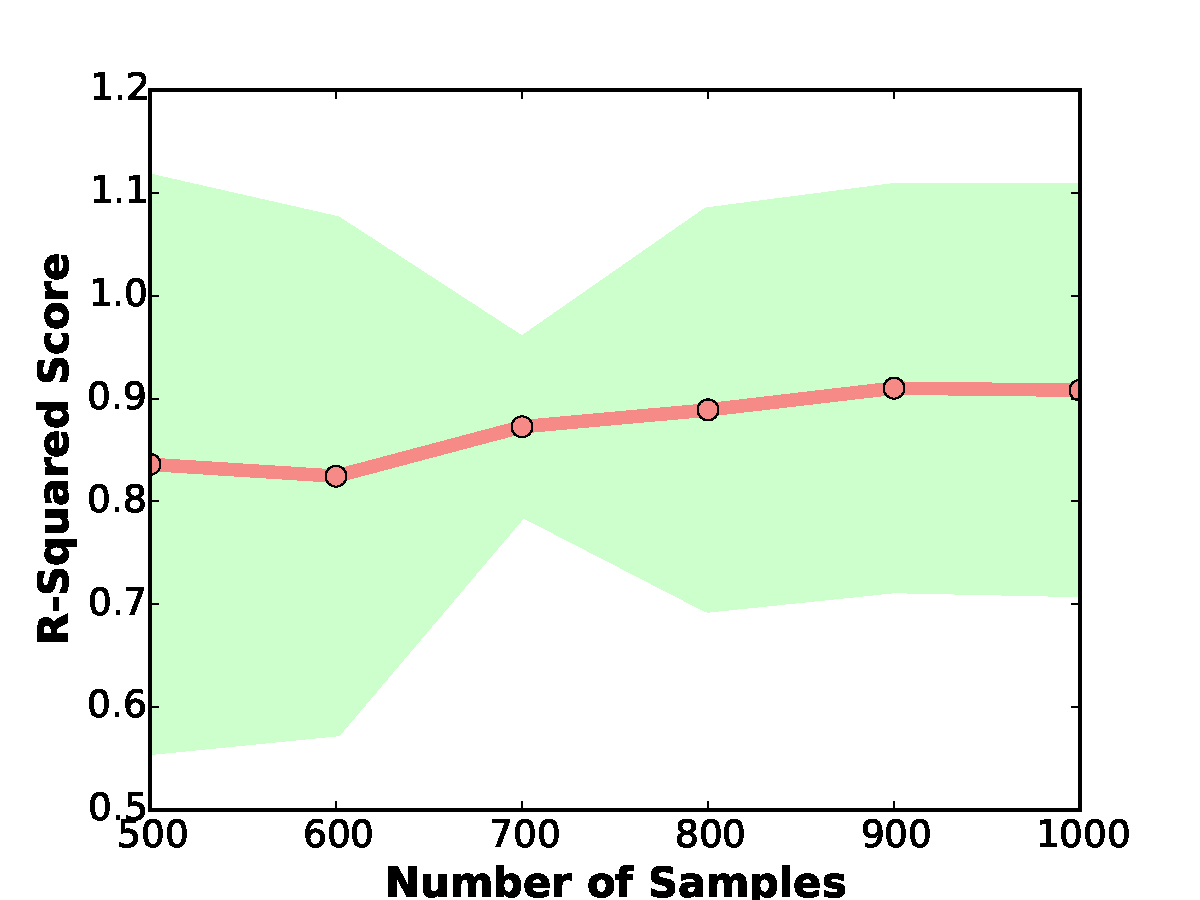
\includegraphics[width=0.5\textwidth]{figure/gp_per_benchmark_r2_scores_throughput_mutate.pdf}}

\caption{Per-benchmark gaussian processes to estimate (a) latency and
  (b) throughput}
\label{fig:gp_r2}
\end{figure*}

% \begin{figure}[h!]
%     \centering
%     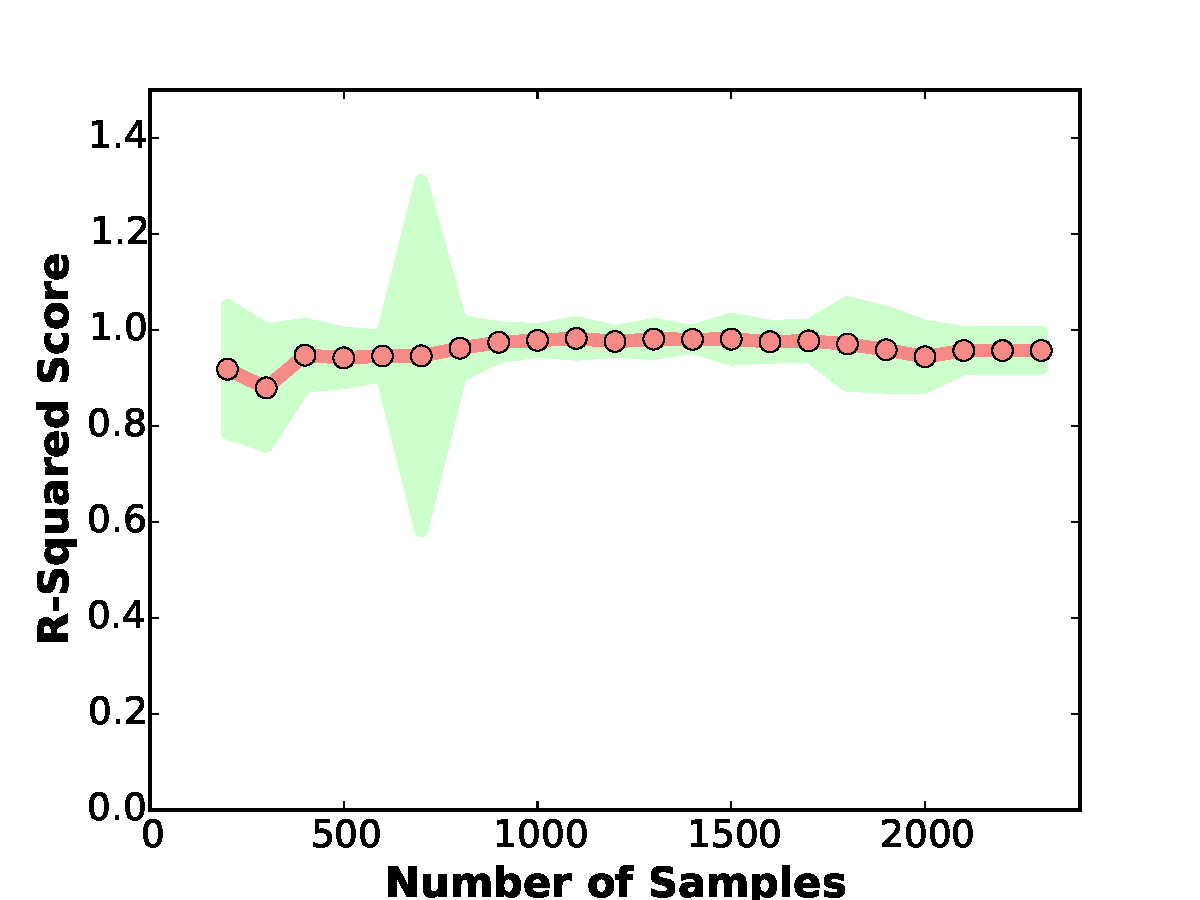
\includegraphics[width=0.7\linewidth]{figure/gp_per_benchmark_r2_scores_latency_mutate.pdf}
%     \caption{Per-benchmark gaussian processes to estimate latency}
%     \label{fig:gp_r2_latency}
% \end{figure}

% \begin{figure}[h!]
%     \centering
%     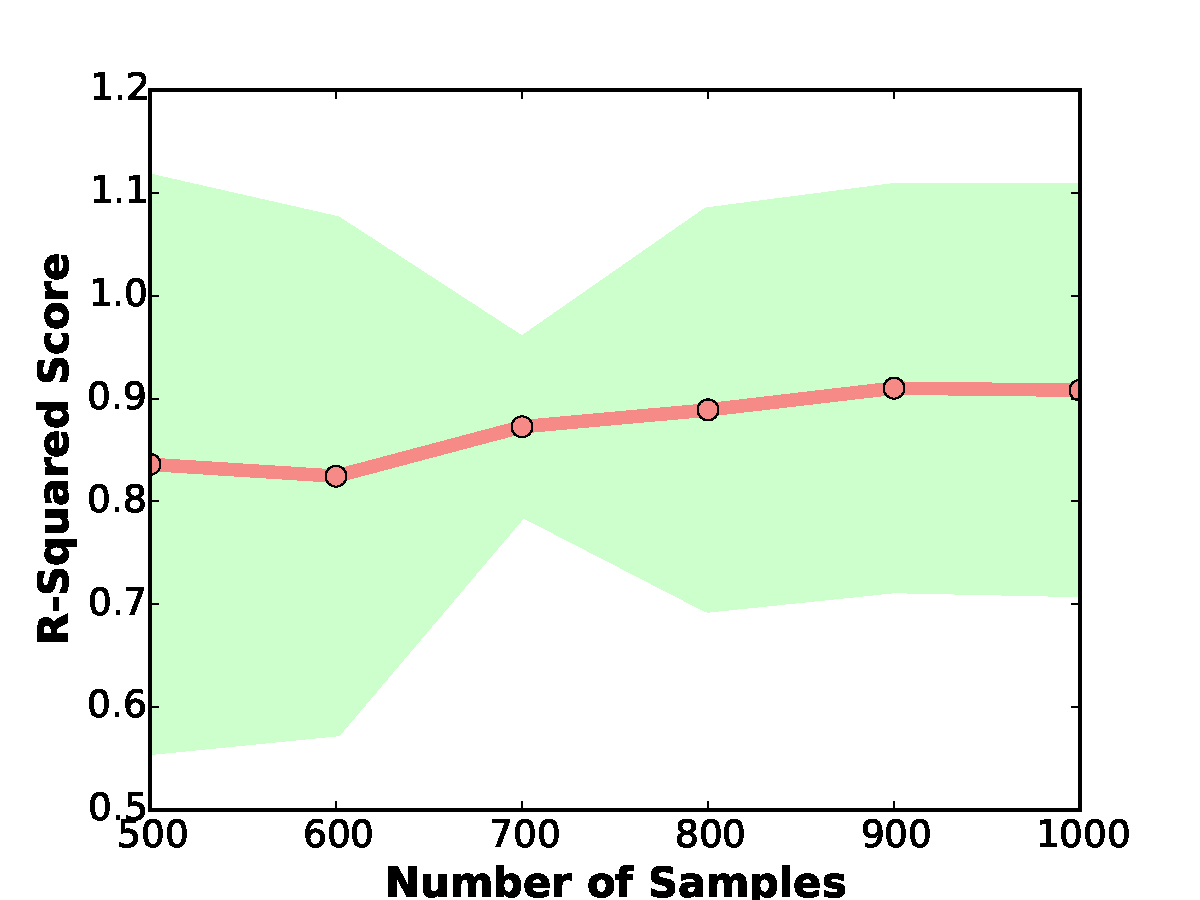
\includegraphics[width=0.7\linewidth]{figure/gp_per_benchmark_r2_scores_throughput_mutate.pdf}
%     \caption{Per-benchmark gaussian processes to estimate throughput}
%     \label{fig:gp_r2_throughput}
% \end{figure}

\begin{figure*}
\subfloat[\label{fig:actual_latency_wikipedia}]{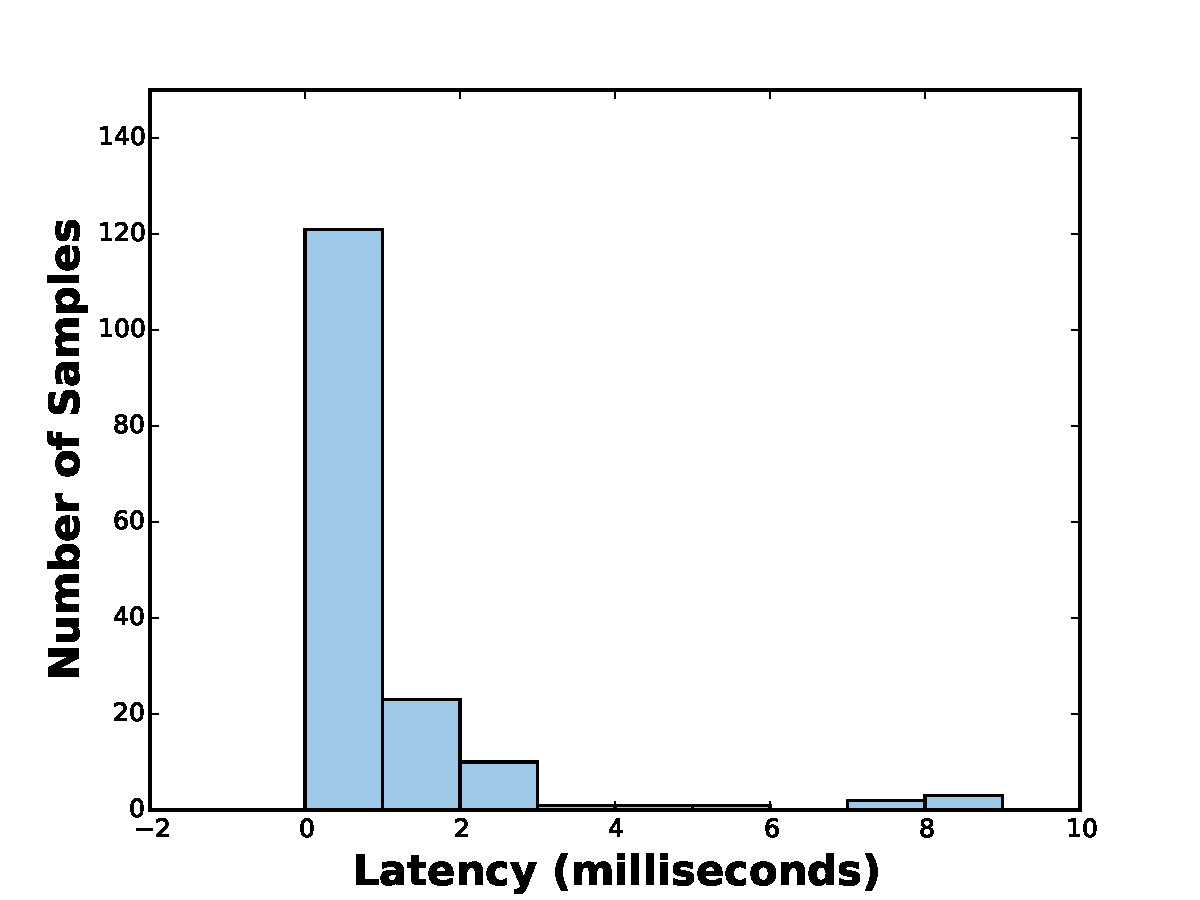
\includegraphics[width=0.5\linewidth]{figure/wikipedia_test_hist_latency_mutate.pdf}}
\subfloat[\label{fig:predicted_latency_wikipedia}]{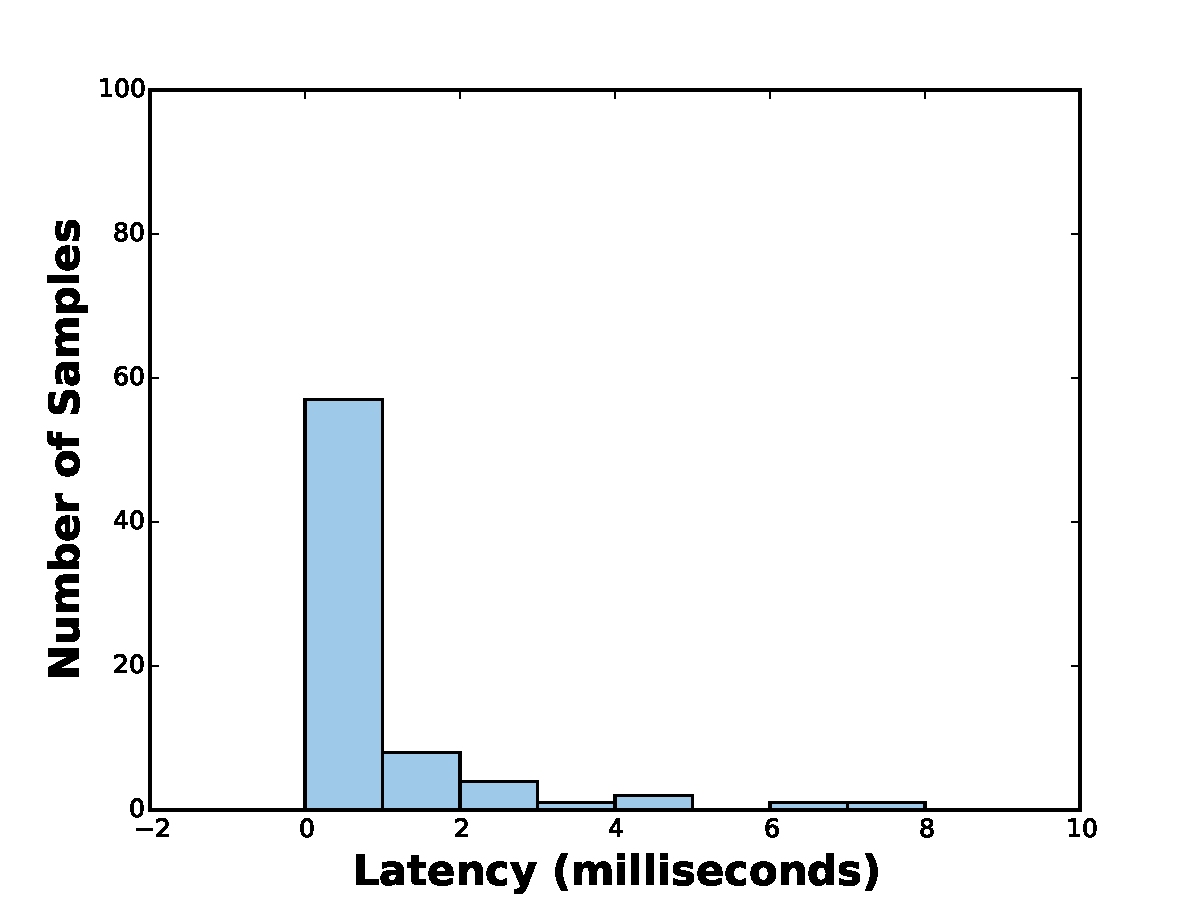
\includegraphics[width=0.5\linewidth]{figure/wikipedia_pred_hist_latency_mutate.pdf}}

\caption{(a) Actual and (b) predicted latency distribution for the
  Wikipedia benchmark}
\label{fig:latency_wikipedia}
\end{figure*}

% \begin{figure}[h!]
%     \centering
%     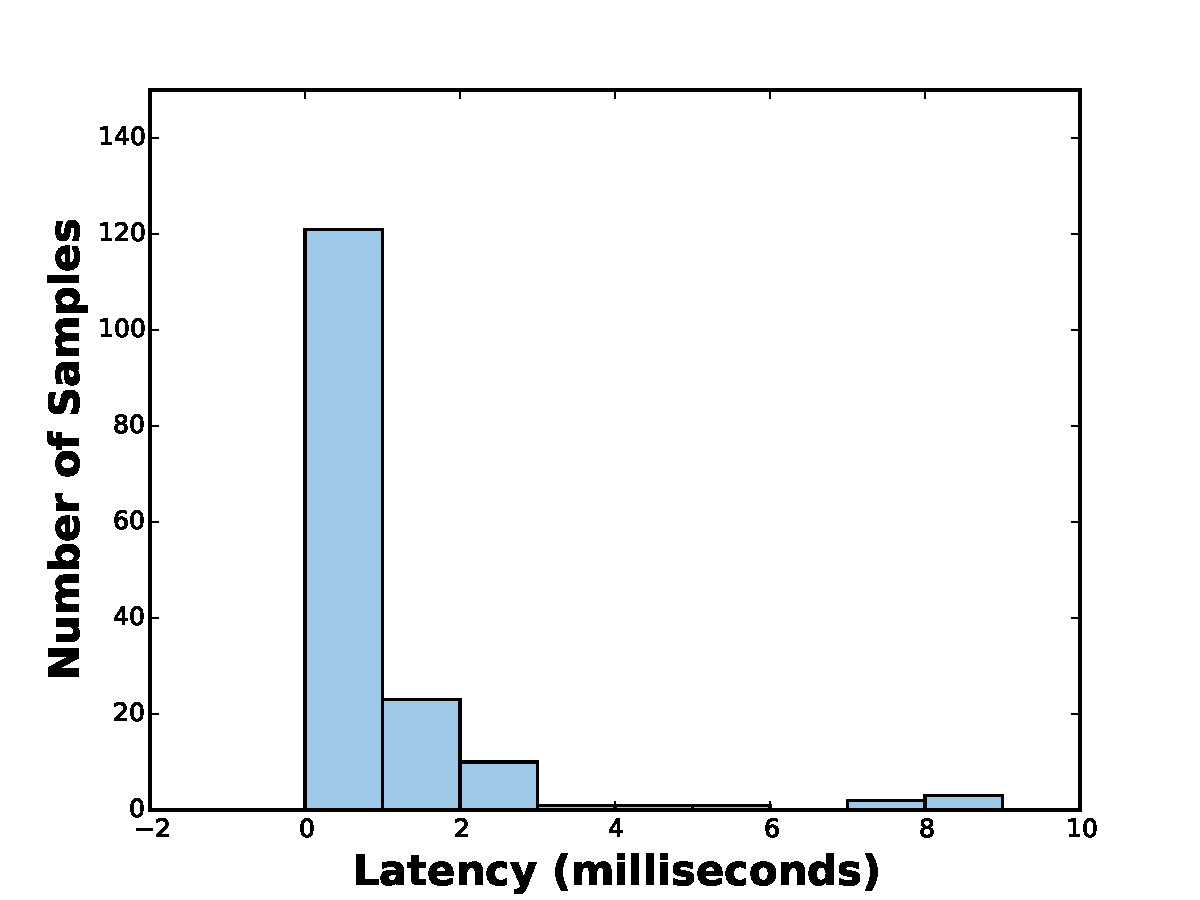
\includegraphics[width=0.7\linewidth]{figure/wikipedia_test_hist_latency_mutate.pdf}
%     \caption{Actual latency distribution for the Wikipedia benchmark}
%     \label{fig:actual_latency_wikipedia}
% \end{figure}

% \begin{figure}[h!]
%     \centering
%     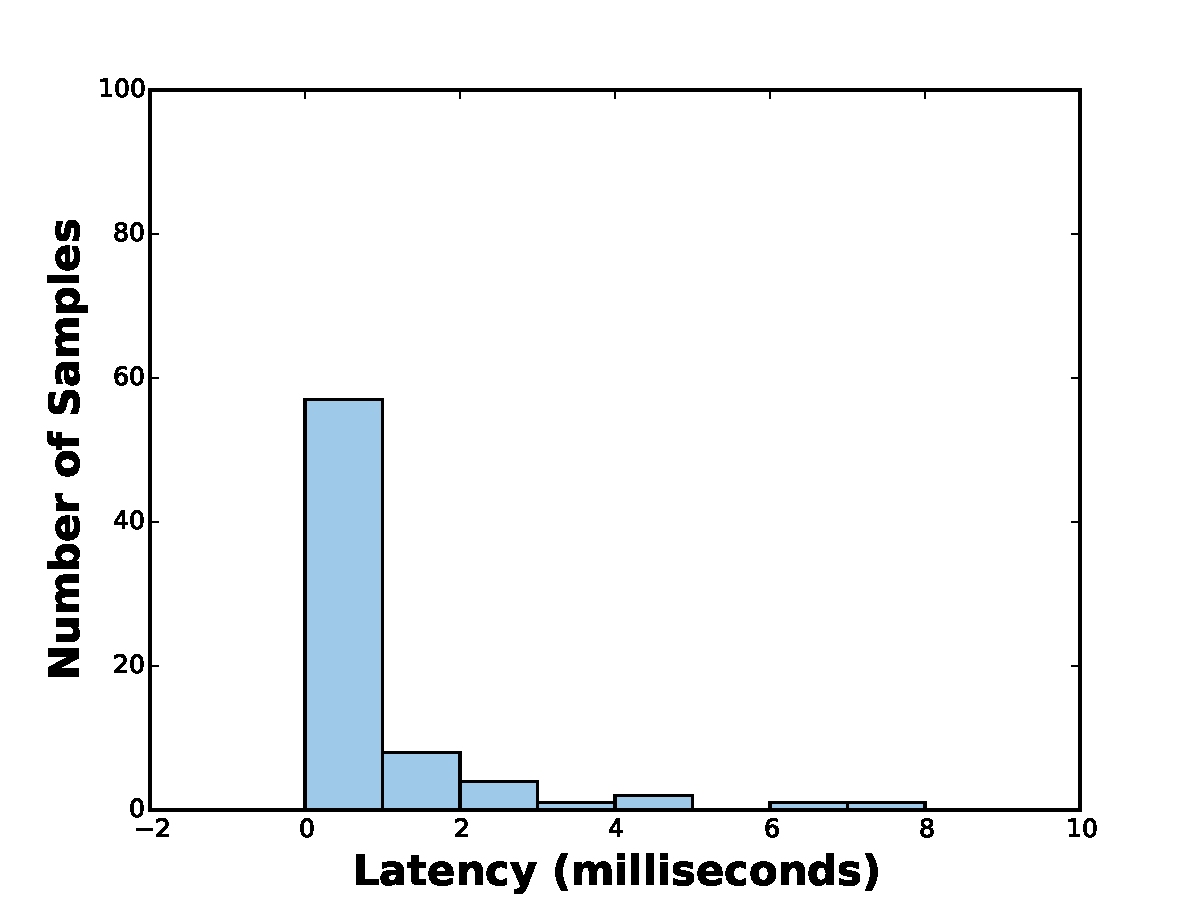
\includegraphics[width=0.7\linewidth]{figure/wikipedia_pred_hist_latency_mutate.pdf}
%     \caption{Predicted latency distribution for the Wikipedia benchmark}
%     \label{fig:predicted_latency_wikipedia}
% \end{figure}

\begin{figure*}
\subfloat[\label{fig:actual_throughput_ycsb_balanced}]{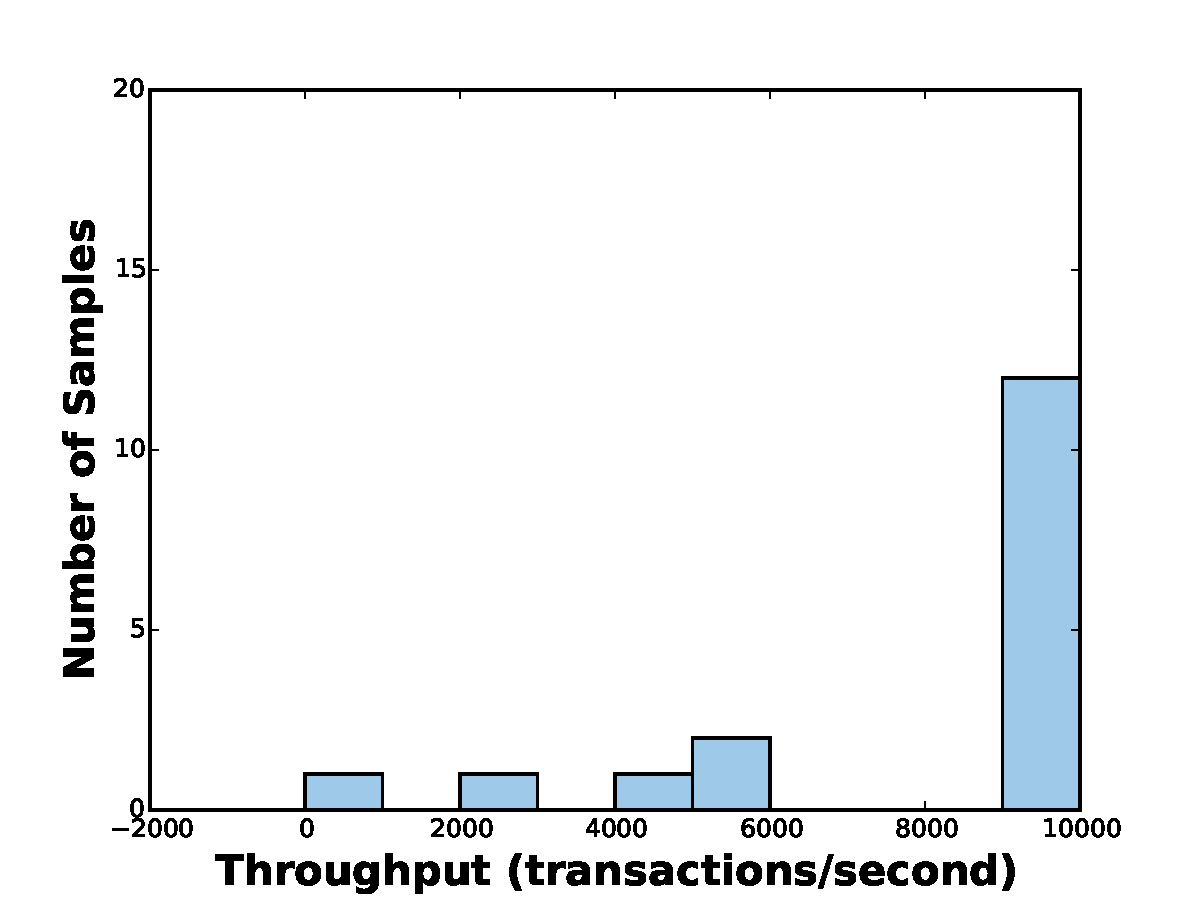
\includegraphics[width=0.5\linewidth]{figure/ycsb_balanced_test_hist_throughput_mutate.pdf}}
\subfloat[\label{fig:predicted_throughput_ycsb_balanced}]{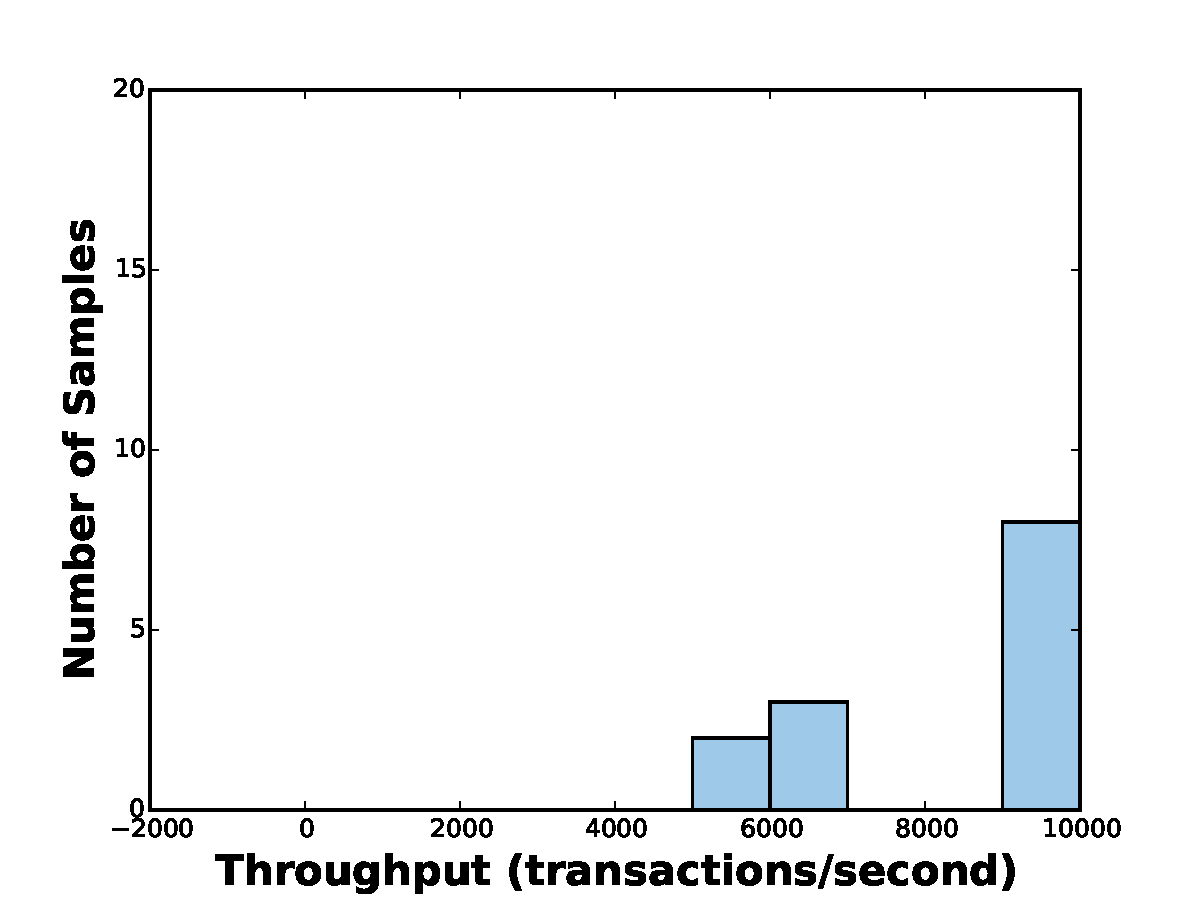
\includegraphics[width=0.5\linewidth]{figure/ycsb_balanced_pred_hist_throughput_mutate.pdf}}

\caption{(a) Actual and (b) predicted throughput distribution for the
  balanced YCSB benchmark}
\label{fig:throughput_ycsb_balanced}
\end{figure*}

% \begin{figure}[h!]
%     \centering
%     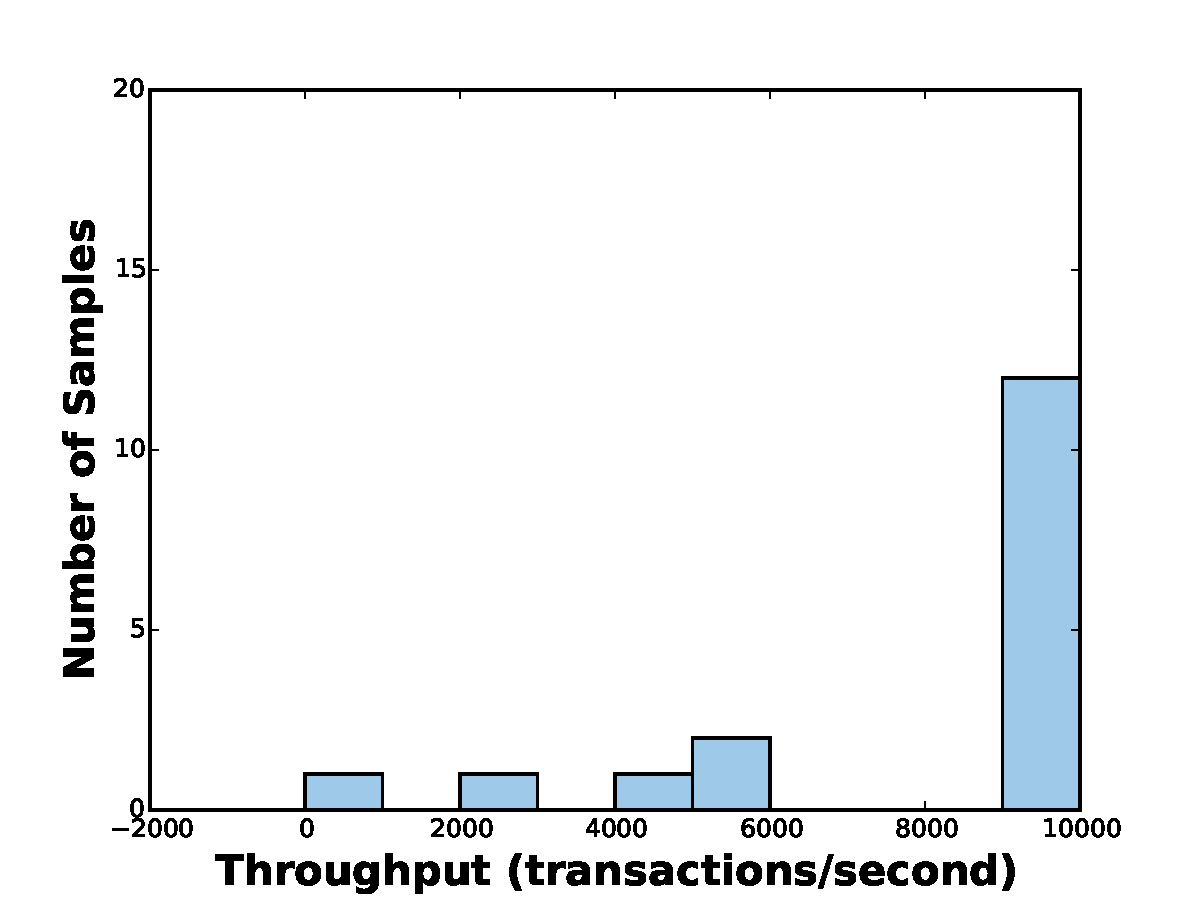
\includegraphics[width=0.7\linewidth]{figure/ycsb_balanced_test_hist_throughput_mutate.pdf}
%     \caption{Actual throughput distribution for the balanced YCSB benchmark}
%     \label{fig:actual_latency_ycsb_balanced}
% \end{figure}

% \begin{figure}[h!]
%     \centering
%     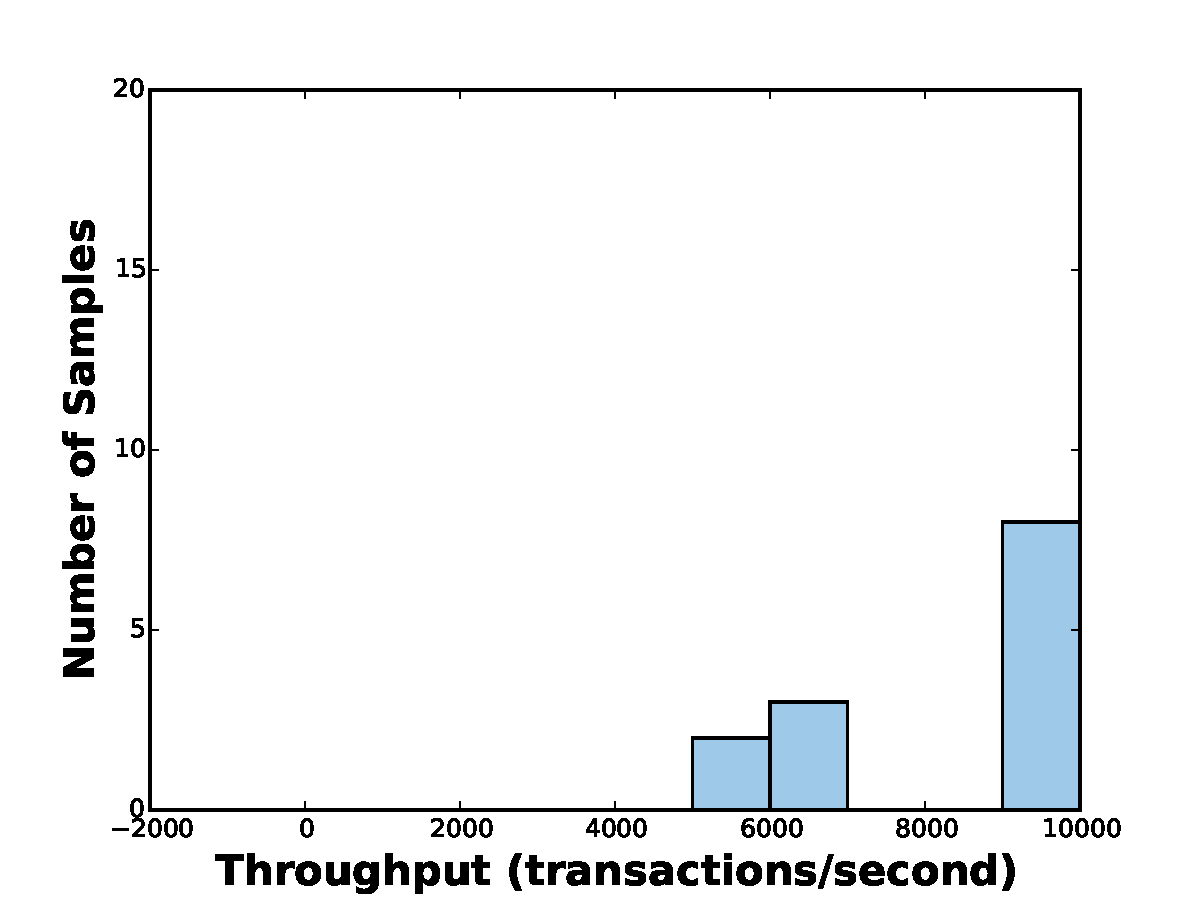
\includegraphics[width=0.7\linewidth]{figure/ycsb_balanced_pred_hist_throughput_mutate.pdf}
%     \caption{Predicted throughput distribution for the balanced YCSB benchmark}
%     \label{fig:predicted_latency_ycsb_balanced}
% \end{figure}

\begin{figure*}
\subfloat[\label{fig:lasso_latency_alphas}]{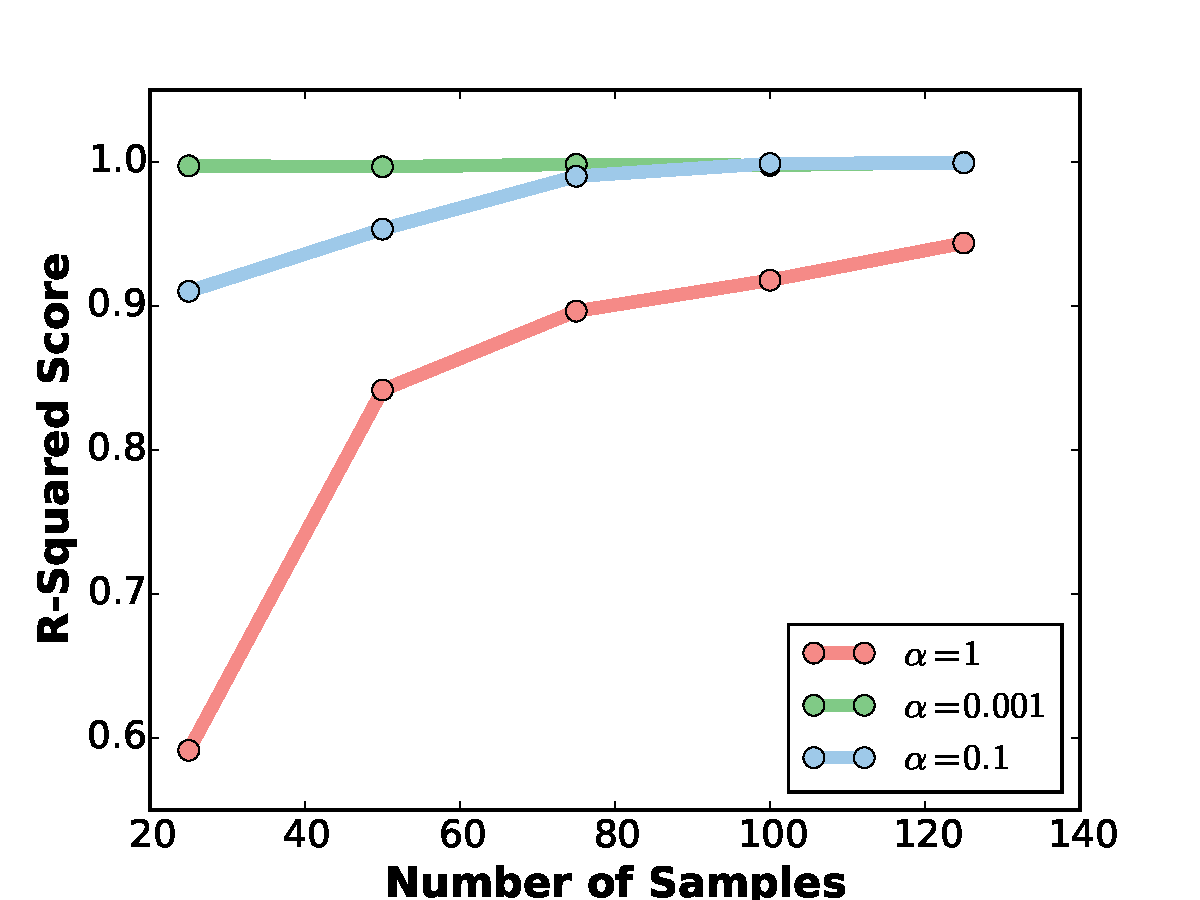
\includegraphics[width=0.5\linewidth]{figure/lasso_latency_mutate.pdf}}
\subfloat[\label{fig:lasso_throughput_alphas}]{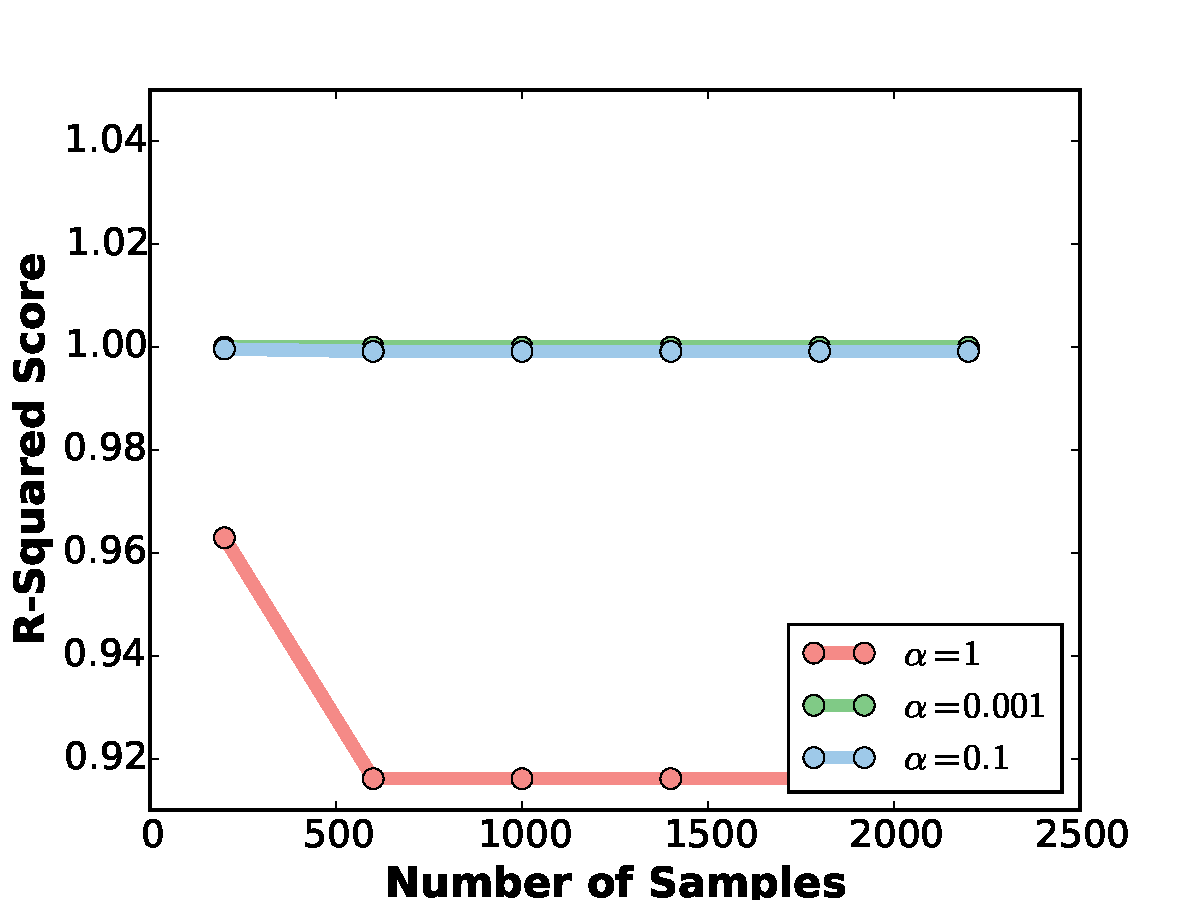
\includegraphics[width=0.5\linewidth]{figure/lasso_throughput_mutate.pdf}}

\caption{Performance of Lasso for various $\alpha$ values for (a)
  latency and (b) throughput on the Wikipedia benchmark}
\label{fig:lasso_alphas}
\end{figure*}

\begin{figure*}
\subfloat[\label{fig:gp_latency_theta0s}]{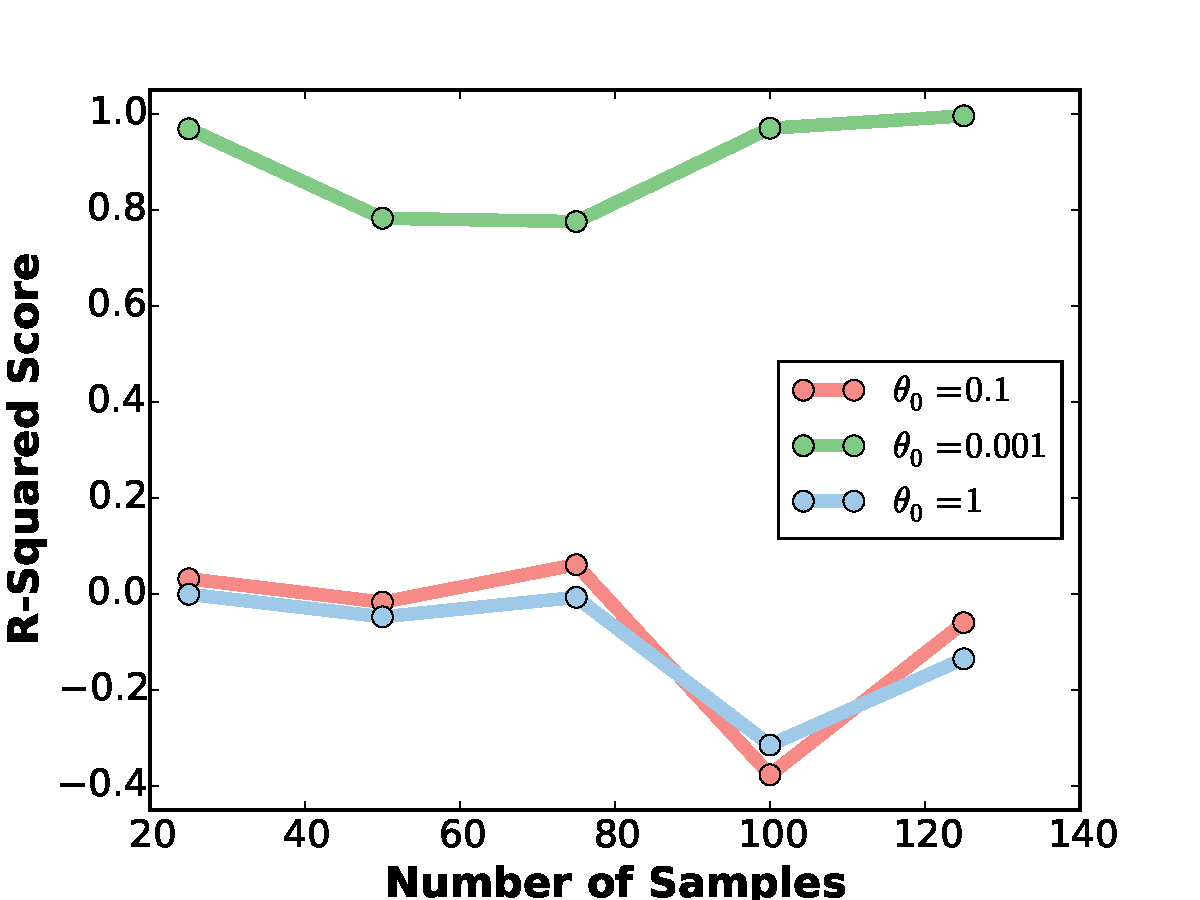
\includegraphics[width=0.5\linewidth]{figure/gp_latency_mutate.pdf}}
\subfloat[\label{fig:gp_throughput_theta0s}]{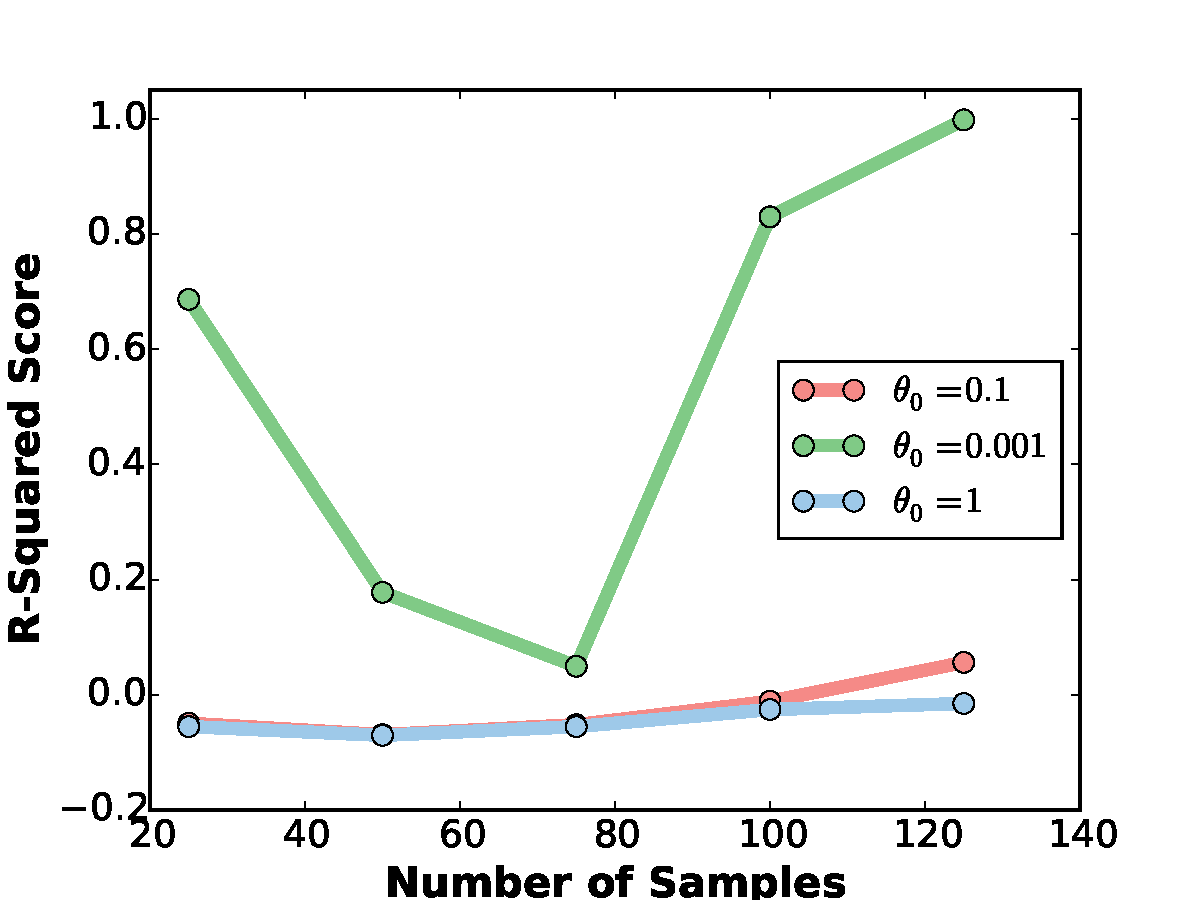
\includegraphics[width=0.5\linewidth]{figure/gp_throughput_mutate.pdf}}

\caption{Performance of Gaussian Process Regression with absolute
  exponential autocorrelation for various $\theta_0$ values for (a)
  latency and (b) throughput on the Wikipedia benchmark}
\label{fig:gp_theta0s}
\end{figure*}

\begin{table*}[h!]
  \centering
  \begin{adjustbox}{max width=0.85\textwidth}
    \begin{tabular}{ll}
      \toprule
      Feature Name                   & Feature Meaning                                                     \\
      \midrule
      PG\_Cache\_Hits                & Number of buffer hits in this table                                 \\
      PG\_Index\_Hits                & Number of buffer hits in all indexes on this table                  \\
      PG\_Index\_scans               & Number of index scans initiated on this
      table                       \\
      PG\_rows\_inserted             & Number of rows inserted by queries in this database                 \\
      PG\_rows\_returned             & Number of rows returned by queries in this database                 \\
      PG\_rows\_updated              & Number of rows updated by queries in this database                  \\
      PG\_sequential\_scans          & Number of sequential scans initiated on this table                  \\
      PG\_transactions\_committed    & Number of transactions in this database that have been committed    \\
      PG\_transactions\_rolled\_back & Number of transactions in this database that have been rolled back  \\
      autovacuum                     & Number of times the autovacuum daemon vacuumed this table           \\
      commit\_delay                  & Time delay before a transaction attempts to flush the WAL buffer    \\
      fsync                          & Enable making sure that updates are physically written to disk      \\
      shared\_buffers                & Amount of memory the database server uses for shared memory buffers \\
      track\_activities              & Enable the collection of information on the executing commands      \\
      wal\_buffers                   & Amount of shared memory used for WAL data                           \\
      wal\_level                     & Determine how much information is written to the WAL                \\
      wal\_writer\_delay             & Specify the delay between activity rounds for the WAL writer        \\
      \bottomrule
    \end{tabular}
  \end{adjustbox}

  \caption{Some of the influential features for throughput estimation.}
  \label{tab:influential_features_for_throughput}
\end{table*}

\begin{table*}[h!]
  \centering
  \begin{adjustbox}{max width=0.85\textwidth}
    \begin{tabular}{ll}
      \toprule
      Feature Name          & Feature Meaning                                                    \\
      \midrule
      PG\_index\_scans      & Number of index scans initiated on this table                      \\
      PG\_sequential\_scans & Number of sequential scans initiated on this table                 \\
      fsync                 & Enable making sure that updates are physically written to disk     \\
      synchronous\_commit   & Whether transaction commit will wait for WAL records to be flushed \\
      \bottomrule
    \end{tabular}
  \end{adjustbox}

  \caption{Influential features for latency estimation.}
  \label{tab:influential_features_for_latency}
\end{table*}

We estimate expected performance of each benchmark on a given database
configuration for the second phase of our solution. In doing so, we
hope to approximately estimate the performance of the target workload
through the estimation for the benchmark it maps to. As such, we train
two estimators for each benchmark: one for database throughput and one
for database latency.

We chose to use Gaussian Process Regression, a supervised learning
method, for this task as it works well for estimating regressions with
no prior knowledge about distribution. It also gives a probabilistic
estimation, allowing for further insight about bounds and probability
of exceeding them. The Gaussian Process Regression models the data
with the function
\begin{equation*}
G(X) = f(X)^{\textrm{T}}\beta + Z(X)
\end{equation*}
where $f(X)^{\textrm{T}}\beta$ is a linear regression model and $Z(X)$
is a Gaussian process with zero mean. $X$ is the input, represented as
a vector of feature values.  In this model, we try to find the ``best
linear unbiased prediction'' (BLUP) of the process given the training
data. That is, we try to find the best function for
$\hat{G}(X) = G(X|\textrm{training data})$. Under the model, it can be
shown that $\hat{G}(X) = a(X)^{\textrm{T}}y$ where $a(X)$ is the
product of the weights with the feature values. From this model, we
can find the we can find the BLUP by solving the optimization problem
\begin{equation*}
a(X)^* = \arg \min\limits_{a(X)} \mathbb{E}[(G(X) - a(X)^T y)^2]
\end{equation*}
subject to the constraint $\mathbb{E}[G(X) - a(X)^T y] = 0$. Gaussian
Processes are amenable to kernels, although they are used as
correlations in this model. We use the absolute exponential
autocorrelation model in our experiments. This covariance model
calculates autocorrelation of a vector X as
\begin{equation*}
  \exp\left( \sum_{i = 1}^n -\theta_0 |\Delta X_i| \right)
\end{equation*}
where $\theta_0$ is a the autocorrelation parameter and $\Delta X$ is
the component-wise distances at which the correlation should be
calculated. We experimented with various values of $\theta_0$ and
settled on $\theta_0 = 0.001$ as it exhibited the best performance, as
seen in \cref{fig:gp_theta0s}.

One way to measure the performance of a regression model is the
$\textrm{R}^2$ score defined as
\begin{equation*}
  \textrm{R}^2 \equiv 1 - \frac{\textrm{SS}_{res}}{\textrm{SS}_{tot}}
\end{equation*}
In this definition, $\textrm{SS}_{res} = \sum_i (y_i - f_i)^2$ where
$y_i$ is the true value and $f_i$ is the predicted value. This term is
also known as the residual sum of squares. The other term in the
definition is $\textrm{SS}_{tot} = \sum_i (y_i - \bar{y})^2$ where
$y_i$ is the true value and $\bar{y}$ is the mean of all the true
values. This is proportional to the variance of the true values. From
this definition of the $\textrm{R}^2$ score, we see that the maximum
value is 1 and that it indicates that the model perfectly predicted
the observed data. A score less than 1 indicates that the model was
not perfect and a score of zero indicates that the model is no better
at predicting the values than the mean of the true
values. \cref{fig:gp_r2} shows
the median $\textrm{R}^2$ score across the estimators for all
benchmarks as a red line. The shaded green region indicates a single
standard deviation spread. We infer from the figures that we can
achieve a very good estimation with as few as 600 samples. In
addition, the estimators become collectively better as more data is
provided, as evidenced by the shrinking green region as number of
samples increases.

One example of a good performance estimator is the latency estimator
for the Wikipedia benchmark. This estimator has a high $\textrm{R}^2$
score of 0.9734. Looking at the actual and predicted latency values in
\cref{fig:latency_wikipedia}, we find that the
predicted distribution mimics the actual one very closely, with only a
slight dip into negative latency predictions. We believe this
estimator can be even stronger if we encode constraints for possible
predictions, such as positive values only.

One example of a poorer performance estimator is the throughput
estimator for the balanced YCSB benchmark. This estimator has a lower
$\textrm{R}^2$ score of 0.7090. Looking at the actual and predicted
throughput values in \cref{fig:throughput_ycsb_balanced}, we see that
the estimator fails to handle the holes in throughput seen in the
actual values. We believe these isolated throughput values are due to
environmental factors that are not reflected in the feature set such
as load on the machine and other processes' resource usages. A more
``global'' set of features across the whole system rather than just
pertaining to the database may help train better estimators.

To gain more insight about what parameters affected performance the
most, we performed Lasso Regression to determine the most influential
features. Lasso regression encourages sparse coefficients in its
solution, so it is a good method for finding the most important
features for a particular problem. It works by optimizing the
objective function
\begin{equation*}
  \min\limits_{w}
  \frac{1}{2n_{\textrm{samples}}} \|Xw - y\|_2^2 + \alpha \|w\|_1
\end{equation*}
which is a simple least squares linear regression with the lasso
constraint added under weight $\alpha$. A higher value for $\alpha$
encourages sparser solutions while a lower value relaxes this
constraint. We experimented with different values of alpha and settled
on using $\alpha = 0.001$ as it exhibited the best performance, as seen in
\cref{fig:lasso_alphas}.

 These features are summarized in
\cref{tab:influential_features_for_throughput} and
\cref{tab:influential_features_for_latency}. Confirming general
intuition, throughput seems to be greatly affected by all operation
types along with options that add delays (e.g. bgwriter\_delay,
commit\_delay) or constrain how relaxed the database can be about
transaction execution (e.g. fsync, synchronous\_commit). However, it
is interesting to note that latency seems primarily affected only by
operations that take a long time to complete and not the type of
operations or hard delays introduced into the system.

In a practical implementation of our estimator, we will not be able
to collect performance statistics before estimating performance for
different configurations. As such, we eliminated the features
pertaining to throughput and latency from consideration. However,
these features are available in the training data. We believe that a
better learner will use graphical models to infer the missing
throughput and performance information for the test data before
estimation. We will explore this technique in the future.